\documentclass[11pt,a4paper]{article}
\usepackage[T1]{fontenc}
\usepackage[utf8]{inputenc}
\usepackage{lmodern}
\usepackage[margin=20mm]{geometry}
\usepackage{graphicx,float}
\usepackage[font=small,labelfont=bf]{caption}
\usepackage[hidelinks]{hyperref}
\graphicspath{{../figures/}}
\setlength{\parindent}{0pt}
\setlength{\parskip}{4pt}
\setlength{\intextsep}{8pt}

\begin{document}
\begin{center}
{\Large\bfseries DT081A --- Laboratory 2 Report\par}
Student: Jakob Obid\par
2026-11-05
\end{center}

\section{Introduction}
This lab studies signals in the time and frequency domains. The tasks include windowing, LTI systems, digital filters and voice analysis.

\section{Experimental Setup}
I used Python with NumPy, SciPy and Matplotlib. For the first task, I sampled three cosine waves at 250 Hz for 0.6 seconds. Their frequencies were 50, 55 and 120 Hz.
I compared rectangular, Hann and Hamming windows using the same signal.
I also tested FIR and IIR systems using unit impulses.

\section{Results and Analysis}
\subsection{Time-Domain Analysis}
The signal contains three cosine waves. The FFT shows peaks at 50, 55 and 120 Hz (Figure~\ref{fig:signal-fft}).

\subsubsection*{Q1. Why does the amplitude spectrum contain negative frequencies?}
\textbf{Answer:} The signal contains real cosine waves, so its FFT has matching positive and negative frequencies. The negative side is a mirror of the positive side. It does not mean extra frequencies were added to the signal (Figure~\ref{fig:signal-fft}).

\begin{figure}[H]
\centering
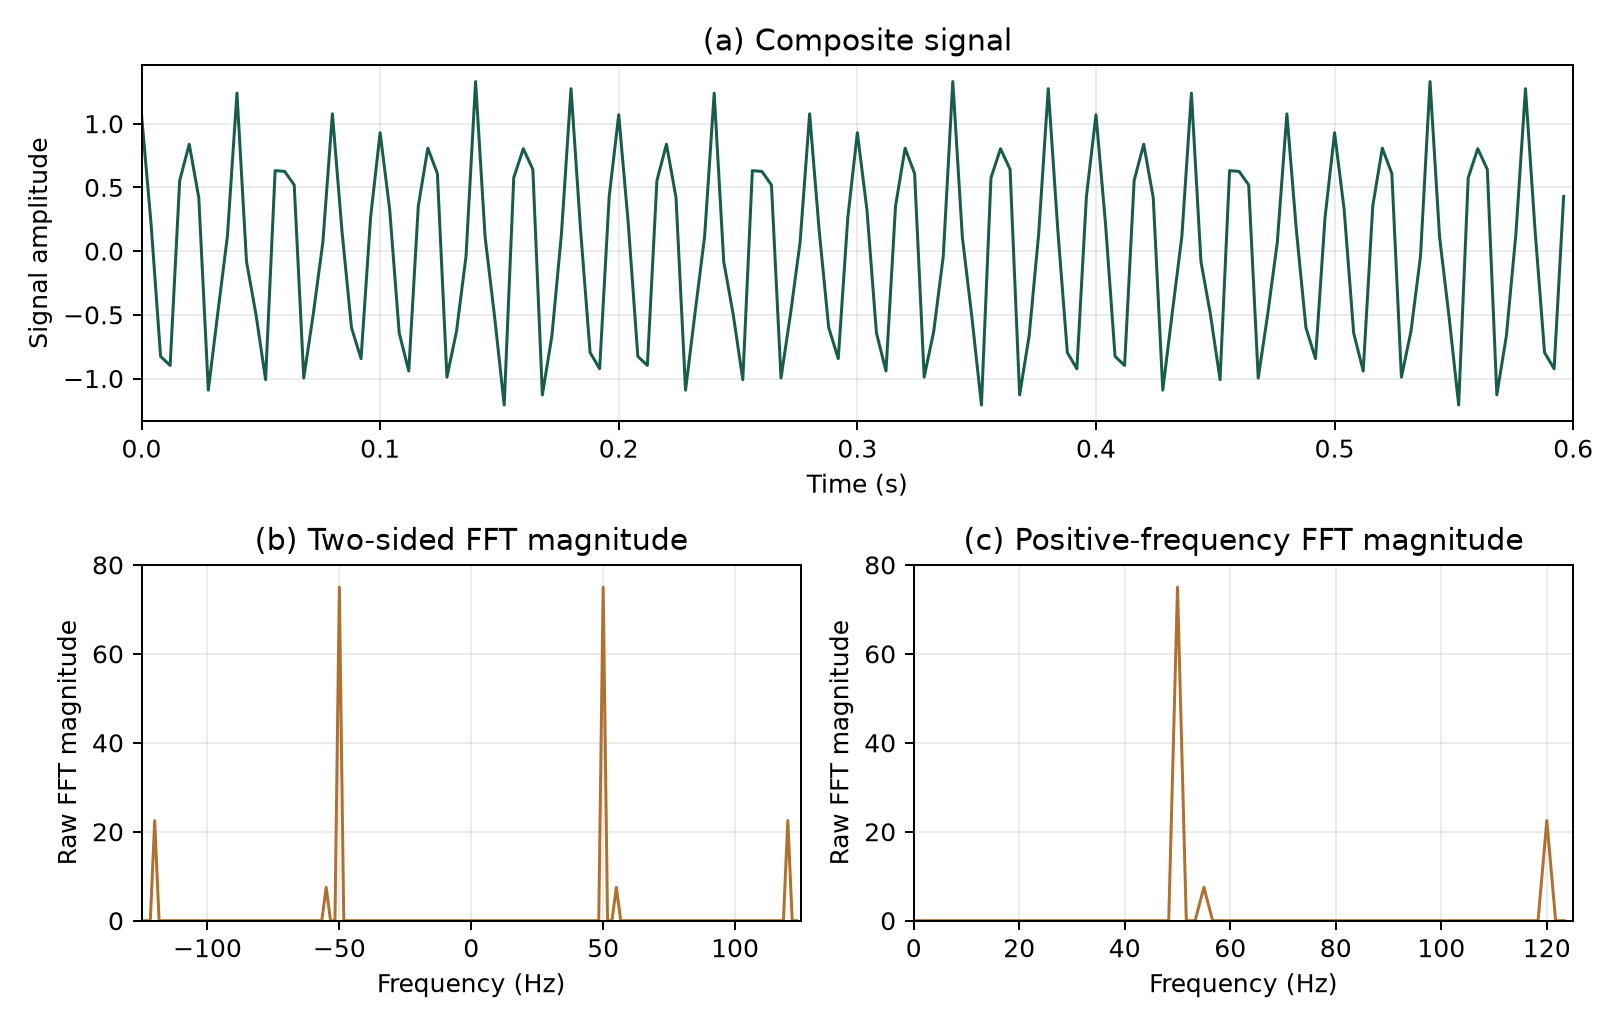
\includegraphics[width=0.95\linewidth]{section1_signal_fft.png}
\caption{Composite signal, two-sided FFT magnitude and positive-frequency FFT magnitude. FFT magnitudes are unnormalized.}
\label{fig:signal-fft}
\end{figure}

\subsection{Frequency Identification}
\subsubsection*{Q1. Which of the windows (rectangular, Hann, and Hamming) is best able to separate frequencies close to each other? Why?}
\textbf{Answer:} The rectangular window separated the 50 Hz and 55 Hz frequencies most clearly in this test. Both frequencies fall exactly on FFT points, so the peaks stay narrow. Hann and Hamming made the peaks wider, but they can reduce leakage when frequencies do not fall exactly on FFT points (Figure~\ref{fig:window-comparison}).

\begin{figure}[H]
\centering
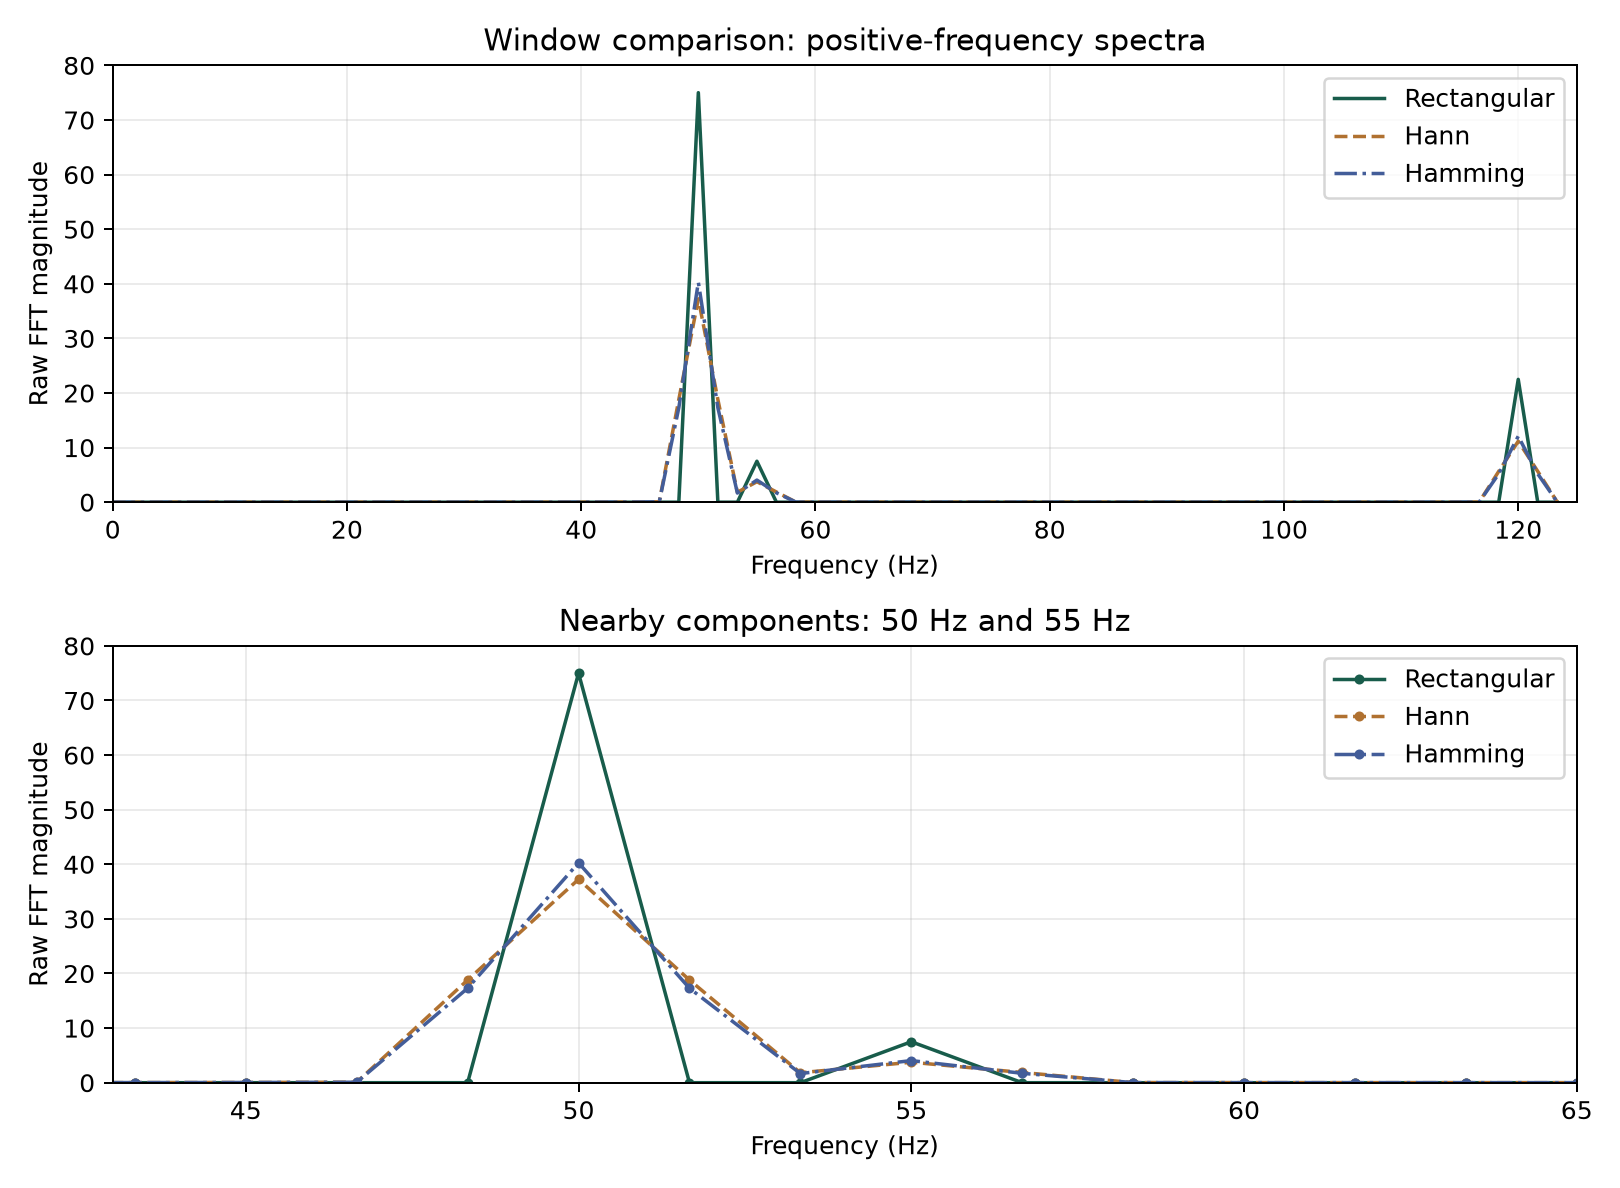
\includegraphics[width=0.95\linewidth]{section2_window_comparison.png}
\caption{Rectangular, Hann and Hamming window spectra. The lower plot zooms in on the 50 Hz and 55 Hz components.}
\label{fig:window-comparison}
\end{figure}

\subsection{Linear Time-Invariant Systems}
\subsubsection*{System 1}

\textbf{Q1. Does the convolution give the correct response?}

\textbf{Answer:} Yes. I convolved the filter coefficients with a unit impulse. The first eight output samples matched the given coefficients, and the remaining samples were zero (Figure~\ref{fig:lti-systems}).

\textbf{Q2. Is this a FIR or IIR system? How can you tell?}

\textbf{Answer:} This is an FIR system because its impulse response ends after eight samples. There is no feedback from earlier output values.

\subsubsection*{System 2}

\textbf{Q1. Implement the system with a loop and plot the output.}

\textbf{Answer:} I used a loop to calculate 100 output samples from a unit impulse. The first five values were 1, -0.3, 0.53, -0.423 and 0.4393 (Figure~\ref{fig:lti-systems}). I followed the supplied filter coefficients, which use the previous two output samples.

The printed difference equation repeats \(y(n-1)\), but the given filter coefficients require \(y(n-2)\) in the final term.

\textbf{Q2. Is this a FIR or IIR system? How can you tell?}

\textbf{Answer:} This is an IIR system because the output depends on earlier output values. Its impulse response continues instead of stopping after a fixed number of samples.

\textbf{Q3. Do you get the same results in the two simulations?}

\textbf{Answer:} Yes. The loop and \texttt{lfilter()} gave the same 100 output values. The maximum difference was zero (Figure~\ref{fig:lti-systems}).

\begin{figure}[H]
\centering
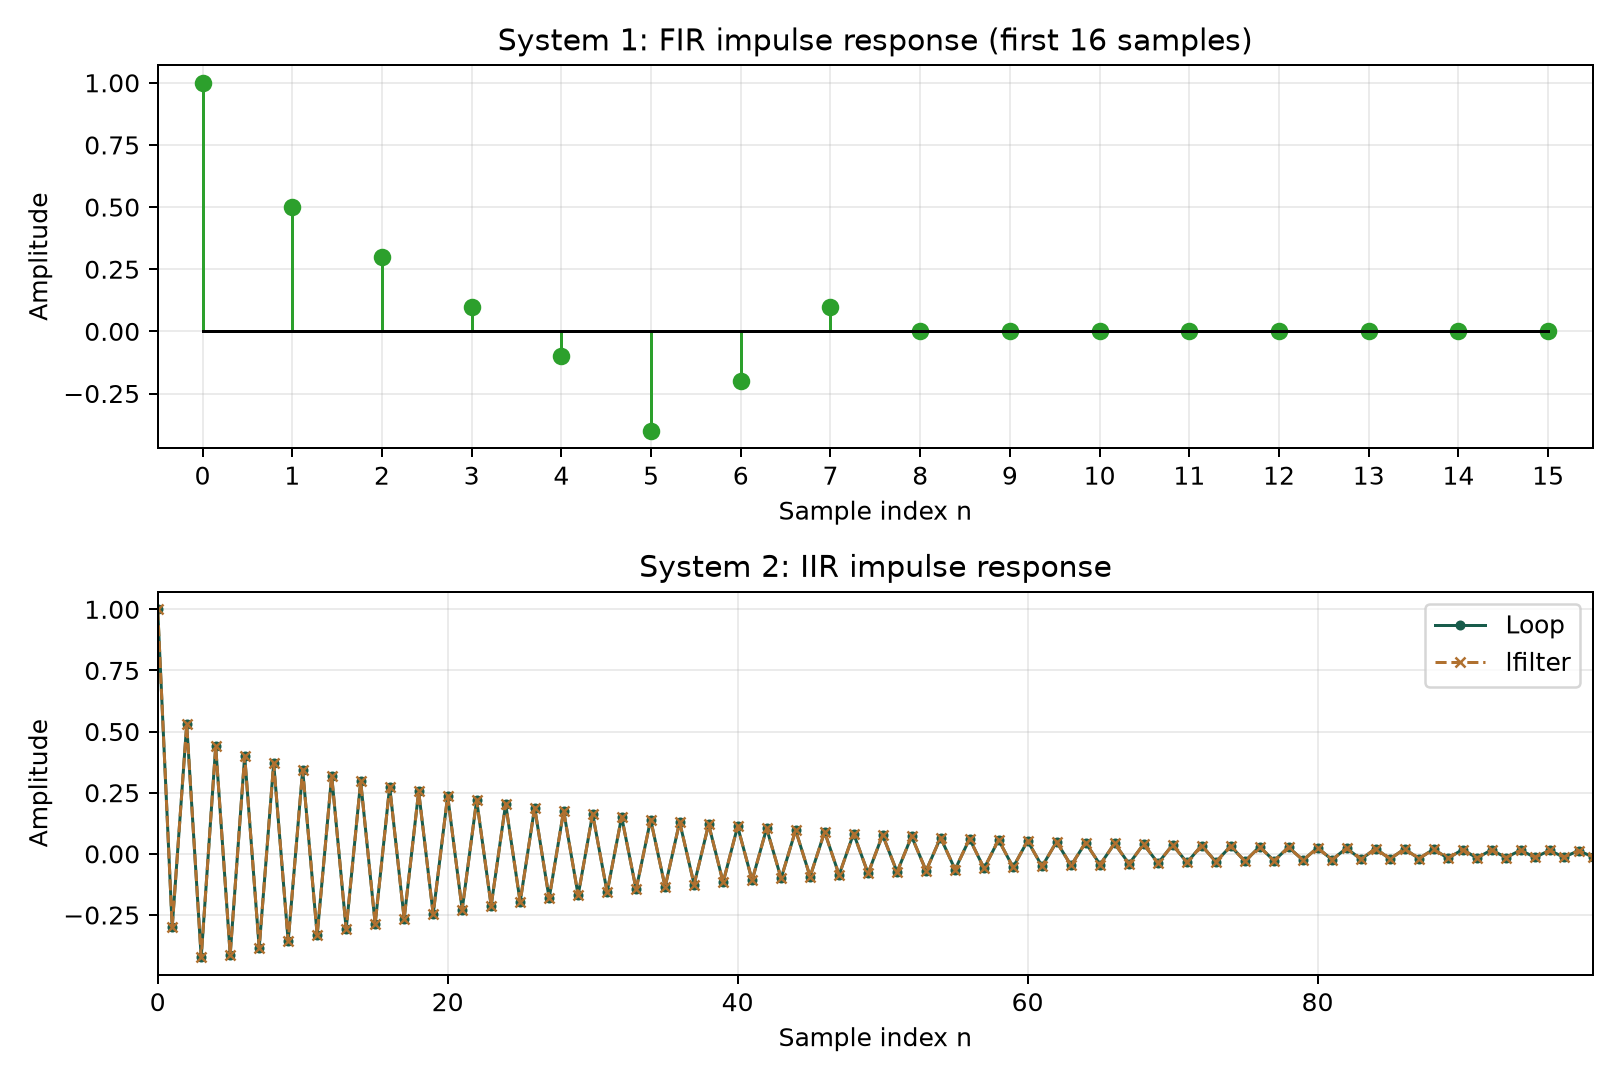
\includegraphics[width=0.95\linewidth]{section3_lti_systems.png}
\caption{Impulse responses of the FIR and IIR systems. The loop and lfilter outputs agree for System 2.}
\label{fig:lti-systems}
\end{figure}

\section{Discussion}
The FFT showed the same frequencies that were used to make the signal. The positive and negative frequency peaks matched because the signal was real.
The rectangular window separated the nearby frequencies best in this test because they matched the FFT frequency points.
The FIR response stopped after eight samples, while the IIR response continued because it uses feedback.

\section{Conclusion}
The first experiment showed how the FFT can identify the frequencies in a signal.
The window comparison showed how different windows change the frequency spectrum.
The two LTI experiments showed the difference between finite and recursive impulse responses.
\end{document}
